\chapter{Cristales II: sólidos iónicos, covalentes y moleculares}\label{ch:b1:crystals-ionic-covalent}

La sal de mesa, al triturarla, se rompe en cubos diminutos; el diamante
es el material natural más duro y, sin embargo, el grafito, hecho de los
mismos átomos de carbono, es lo bastante blando para escribir con él; el
hielo flota en el agua. Todos son \omterm{def:b1:crystals-metals:crystal}{cristales}, pero sus partículas se
mantienen unidas de maneras distintas: los iones, por atracción
electrostática; los átomos, por \omterm{def:b1:lewis-resonance-vsepr:lewis}{enlaces covalentes}; las moléculas, por las
fuerzas intermoleculares del \cref{ch:b1:intermolecular-forces-solvents}.
Este capítulo aplica la geometría de la celda del capítulo anterior a
estas tres familias de sólidos y explica, a partir del tamaño de los
iones, por qué el cloruro de sodio y el cloruro de cesio adoptan
estructuras distintas.

\begin{recall}
La \omterm{def:b1:crystals-metals:multiplicity}{multiplicidad} de una celda, el \omterm{def:b1:crystals-metals:coordination}{número de coordinación} y la \omterm{def:b1:crystals-metals:compactness}{compacidad},
así como los \omterm{def:b1:crystals-metals:site}{huecos octaédricos} y tetraédricos de la \omterm{def:b1:crystals-metals:lattice}{red} \omterm{def:b1:crystals-metals:packings}{cúbica centrada
en las caras}, se definieron en el \cref{ch:b1:crystals-metals}; la
densidad de un \omterm{def:b1:crystals-metals:crystal}{cristal} es $\rho = ZM/(N_A V)$
(\cref{prop:b1:crystals-metals:density}). Los \omterm{def:b1:periodicity:radius}{radios iónicos} se
introdujeron en la \cref{def:b1:periodicity:radius}.
\end{recall}

\section{Cristales iónicos y relación de radios}

\begin{definition}[Cristal iónico]\label{def:b1:crystals-ionic-covalent:ionic-crystal}
Un \emph{cristal iónico}\index{cristal ionico@cristal iónico} es un \omterm{def:b1:crystals-metals:crystal}{cristal} de cationes y
aniones unidos por atracción electrostática. Cada ion está rodeado de
iones de carga opuesta; el \omterm{def:b1:crystals-metals:crystal}{cristal} es eléctricamente neutro, de modo que
los números de cationes y de aniones de una celda están en la proporción
de la fórmula.
\end{definition}

\begin{proposition}[Propiedades de los cristales iónicos]\label{prop:b1:crystals-ionic-covalent:ionic-properties}
Los \omterm{def:b1:crystals-ionic-covalent:ionic-crystal}{cristales iónicos} son duros pero frágiles (un desplazamiento de una
capa enfrenta iones del mismo signo, y el \omterm{def:b1:crystals-metals:crystal}{cristal} se exfolia), tienen
puntos de fusión altos, no conducen en estado sólido pero sí fundidos o
disueltos, y se disuelven en \omterm{def:b1:intermolecular-forces-solvents:solvent-classes}{disolventes polares} de permitividad alta.
\end{proposition}
\admitted

\begin{definition}[Relación de radios]\label{def:b1:crystals-ionic-covalent:radius-ratio}
En un \omterm{def:b1:crystals-ionic-covalent:ionic-crystal}{cristal iónico} de un catión de radio $r_+$ y un anión de radio
$r_-$, la \emph{relación de radios}\index{relacion de radios@relación de radios} es $x = r_+/r_-$
(normalmente $x < 1$, pues los cationes son más pequeños que los
aniones).
\end{definition}

\begin{proposition}[La regla de la relación de radios]\label{prop:b1:crystals-ionic-covalent:rule}
En el modelo de esferas rígidas, una estructura en la que cada catión toca
$n$ aniones solo es estable si los aniones no se tocan entre sí, lo que
exige que $x$ supere un límite fijado por la geometría: $x \ge \sqrt3 - 1
\approx 0.732$ para 8 vecinos (cubo), $x \ge \sqrt2 - 1 \approx 0.414$
para 6 (octaedro), $x \ge \sqrt{3/2} - 1 \approx 0.225$ para 4
(tetraedro). La estructura adoptada es la de mayor coordinación que
permite $x$.
\end{proposition}

\begin{proof}
El catión se sitúa en el hueco entre $n$ aniones en contacto con él. En
el límite, los aniones también se tocan entre sí. Cubo: los aniones están
en los vértices de un cubo de arista $2r_-$ y el catión en su centro, de
modo que $r_+ +
r_- = \sqrt3\,r_-$. Octaedro: cuatro aniones en un cuadrado de lado
$2r_-$, con el catión en su centro, $r_+ + r_- = \sqrt2\,r_-$. Tetraedro:
los aniones en vértices alternos de un cubo de arista $\sqrt2\,r_-$, con
el catión en el centro, $r_+ + r_- = \frac{\sqrt3}{2}\sqrt2\,r_- = \sqrt{3/2}\,r_-$.
Al dividir por $r_-$ se obtienen los límites. Por debajo del límite, el
catión baila en un hueco demasiado grande para él: los aniones se repelen
sin que aumente la atracción, de modo que se prefiere una coordinación
menor, con un hueco más pequeño.
\end{proof}

\begin{omfigure}
\begin{tikzpicture}[font=\small, >={Stealth}]
  \draw[->, thick] (0,0) -- (12.4,0) node[right] {$x = r_+/r_-$};
  \foreach \x/\l in {0/0, 2.7/0.225, 4.97/0.414, 8.78/0.732, 12/1} {
    \draw (\x,0.12) -- (\x,-0.12) node[below] {\l};
  }
  \fill[omDef!15] (2.7,0.2) rectangle (4.97,1.0);
  \fill[omProp!15] (4.97,0.2) rectangle (8.78,1.0);
  \fill[omThm!15] (8.78,0.2) rectangle (12,1.0);
  \node[align=center] at (3.83,0.6) {4: ZnS};
  \node[align=center] at (6.87,0.6) {6: NaCl};
  \node[align=center] at (10.4,0.6) {8: CsCl};
  \foreach \x/\l in {3.91/\ce{ZnS}, 6.76/\ce{NaCl}, 10.08/\ce{RbCl}, 11.54/\ce{CsCl}} {
    \draw[omExo, thick] (\x,-0.55) -- (\x,-0.95);
    \node[below, omExo] at (\x,-0.95) {\l};
  }
\end{tikzpicture}

{\small La regla de la \omterm{def:b1:crystals-ionic-covalent:radius-ratio}{relación de radios}: la coordinación del catión que
permite $x$, y las relaciones medidas de cuatro sales (radios de
Shannon). El cloruro de rubidio, con 0.84, debería ser del tipo \ce{CsCl}
pero adopta el tipo \ce{NaCl}: la regla es una guía, no una ley
(\cref{exo:b1:crystals-ionic-covalent:12}).}
% ledger: rion:Zn2+IV, rion:S2-VI, rion:Na+VI, rion:Cl-VI, rion:Rb+VI,
% rion:Cs+VIII
\end{omfigure}

\section{Cuatro tipos estructurales}

\begin{definition}[Tipos estructurales]\label{def:b1:crystals-ionic-covalent:structure-type}
Los \omterm{def:b1:crystals-ionic-covalent:ionic-crystal}{cristales iónicos} se clasifican en unos pocos tipos estructurales,
que reciben el nombre de un compuesto representativo:
\begin{itemize}
  \item \emph{tipo cloruro de cesio}\index{tipo cloruro de cesio}: aniones
        en los vértices de un cubo y el catión en su centro (8:8);
  \item \emph{tipo sal gema}\index{tipo sal gema} (tipo cloruro de
        sodio): aniones en una \omterm{def:b1:crystals-metals:lattice}{red} FCC y cationes en todos sus \omterm{def:b1:crystals-metals:site}{huecos
        octaédricos} (6:6);
  \item \emph{tipo blenda}\index{tipo blenda}: aniones en una \omterm{def:b1:crystals-metals:lattice}{red} FCC y
        cationes en la mitad de sus \omterm{def:b1:crystals-metals:site}{huecos tetraédricos}, uno de cada dos,
        alternados (4:4);
  \item \emph{tipo fluorita}\index{tipo fluorita}: cationes en una \omterm{def:b1:crystals-metals:lattice}{red} FCC
        y aniones en todos sus \omterm{def:b1:crystals-metals:site}{huecos tetraédricos} (8:4), fórmula
        \ce{MX2}; en el \emph{tipo antifluorita}\index{tipo antifluorita}
        se intercambian los papeles (\ce{Li2O}, 4:8).
\end{itemize}
El par de números da la coordinación del catión y la del anión.
\end{definition}

\begin{omfigure}
\tdplotsetmaincoords{60}{100}
\begin{tikzpicture}[tdplot_main_coords, font=\small]
  \pic {omcubeo={3}};
    \node[aX={green!55!black}{6.5mm}] at (0,0,0) {};
  \node[aX={violet!70}{3.8mm}] at (0,1.5,0) {};
  \node[aX={green!55!black}{6.5mm}] at (0,3,0) {};
  \node[aX={violet!70}{3.8mm}] at (0,0,1.5) {};
  \node[aX={green!55!black}{6.5mm}] at (0,1.5,1.5) {};
  \node[aX={violet!70}{3.8mm}] at (0,3,1.5) {};
  \node[aX={violet!70}{3.8mm}] at (1.5,0,0) {};
  \node[aX={green!55!black}{6.5mm}] at (0,0,3) {};
  \node[aX={green!55!black}{6.5mm}] at (1.5,1.5,0) {};
  \node[aX={violet!70}{3.8mm}] at (0,1.5,3) {};
  \node[aX={violet!70}{3.8mm}] at (1.5,3,0) {};
  \node[aX={green!55!black}{6.5mm}] at (0,3,3) {};
  \node[aX={green!55!black}{6.5mm}] at (1.5,0,1.5) {};
  \node[aX={violet!70}{3.8mm}] at (1.5,1.5,1.5) {};
  \node[aX={green!55!black}{6.5mm}] at (1.5,3,1.5) {};
  \node[aX={green!55!black}{6.5mm}] at (3,0,0) {};
  \node[aX={violet!70}{3.8mm}] at (1.5,0,3) {};
  \node[aX={violet!70}{3.8mm}] at (3,1.5,0) {};
  \node[aX={green!55!black}{6.5mm}] at (1.5,1.5,3) {};
  \node[aX={green!55!black}{6.5mm}] at (3,3,0) {};
  \node[aX={violet!70}{3.8mm}] at (1.5,3,3) {};
  \node[aX={violet!70}{3.8mm}] at (3,0,1.5) {};
  \node[aX={green!55!black}{6.5mm}] at (3,1.5,1.5) {};
  \node[aX={violet!70}{3.8mm}] at (3,3,1.5) {};
  \node[aX={green!55!black}{6.5mm}] at (3,0,3) {};
  \node[aX={violet!70}{3.8mm}] at (3,1.5,3) {};
  \node[aX={green!55!black}{6.5mm}] at (3,3,3) {};
  \node at (1.5,1.5,-1.75) {\ce{NaCl} (sal gema)};
\end{tikzpicture}
\hspace{1cm}
\begin{tikzpicture}[tdplot_main_coords, font=\small]
  \pic {omcubeo={3}};
    \node[aX={green!55!black}{6.5mm}] at (0,0,0) {};
  \node[aX={green!55!black}{6.5mm}] at (0,3,0) {};
  \node[aX={green!55!black}{6.5mm}] at (0,0,3) {};
  \node[aX={green!55!black}{6.5mm}] at (0,3,3) {};
  \node[aX={blue!60}{7mm}] at (1.5,1.5,1.5) {};
  \node[aX={green!55!black}{6.5mm}] at (3,0,0) {};
  \node[aX={green!55!black}{6.5mm}] at (3,3,0) {};
  \node[aX={green!55!black}{6.5mm}] at (3,0,3) {};
  \node[aX={green!55!black}{6.5mm}] at (3,3,3) {};
  \node at (1.5,1.5,-1.75) {\ce{CsCl}};
\end{tikzpicture}

{\small A la izquierda, la celda de la sal gema, con \ce{Cl-} (verde) en
una \omterm{def:b1:crystals-metals:lattice}{red} FCC y \ce{Na+} (violeta) en todos los \omterm{def:b1:crystals-metals:site}{huecos octaédricos}. A la
derecha, la celda del cloruro de cesio, con \ce{Cl-} en los vértices y
\ce{Cs+} (azul) en el centro. Los iones se dibujan más pequeños que en
contacto.}
\end{omfigure}

\begin{proposition}[Tipos sal gema y cloruro de cesio]\label{prop:b1:crystals-ionic-covalent:nacl-cscl}
En el \omterm{def:b1:crystals-ionic-covalent:structure-type}{tipo sal gema} hay $Z = 4$ unidades fórmula por celda, los iones se
tocan a lo largo de una arista, $a = 2(r_+ + r_-)$, y la estructura exige
$\sqrt2 - 1
\le x$. En el \omterm{def:b1:crystals-ionic-covalent:structure-type}{tipo cloruro de cesio}, $Z = 1$, los iones se tocan a lo
largo de la diagonal principal, $a\sqrt3 = 2(r_+ + r_-)$, y la estructura
exige $x \ge \sqrt3 - 1$.
\end{proposition}

\begin{proof}
Sal gema: los aniones de la \omterm{def:b1:crystals-metals:lattice}{red} FCC cuentan $4$, y los cationes de los 4
\omterm{def:b1:crystals-metals:site}{huecos octaédricos}, $1 + 12 \times \frac14 = 4$. A lo largo de una arista
se suceden en contacto anión, catión y anión. Los aniones no se solapan
si la diagonal de cara, que contiene tres aniones de los que a lo sumo
dos se tocan, cumple $a\sqrt2 \ge 4r_-$, es decir, $2(r_+ + r_-)\sqrt2 \ge
4r_-$, o $x \ge \sqrt2 - 1$. Cloruro de cesio: $8 \times \frac18 = 1$
anión y 1 catión; en la diagonal principal, anión, catión y anión en
contacto; los aniones no se solapan a lo largo de una arista si
$a \ge 2r_-$, es decir,
$2(r_+ + r_-)/\sqrt3 \ge 2r_-$, o $x \ge \sqrt3 - 1$.
\end{proof}

\begin{example}[Cloruro de sodio y cloruro de cesio]\label{ex:b1:crystals-ionic-covalent:nacl}
El cloruro de sodio tiene $a = \qty{564.1}{pm}$: $r_+ + r_- = a/2 =
\qty{282.0}{pm}$, frente a $102 + 181 = \qty{283}{pm}$ según los radios de
Shannon; $x = 102/181 = 0.56$, en el intervalo octaédrico. Su densidad es
$\rho = 4 \times 58.44/(6.022 \times 10^{23} \times (5.641 \times
10^{-8})^3) = \qty{2.16}{g/cm^3}$, y la medida, \qty{2.17}{g/cm^3}. El
cloruro de cesio tiene $a = \qty{412.3}{pm}$: $r_+ + r_- = a\sqrt3/2 =
\qty{357.1}{pm}$, y $x = 174/181 = 0.96$, en el intervalo cúbico.
% ledger: lat:NaCl, rion:Na+VI, rion:Cl-VI, rho:NaCl, lat:CsCl,
% rion:Cs+VIII
\end{example}

\begin{omfigure}
\begin{minipage}[b]{0.31\linewidth}\centering
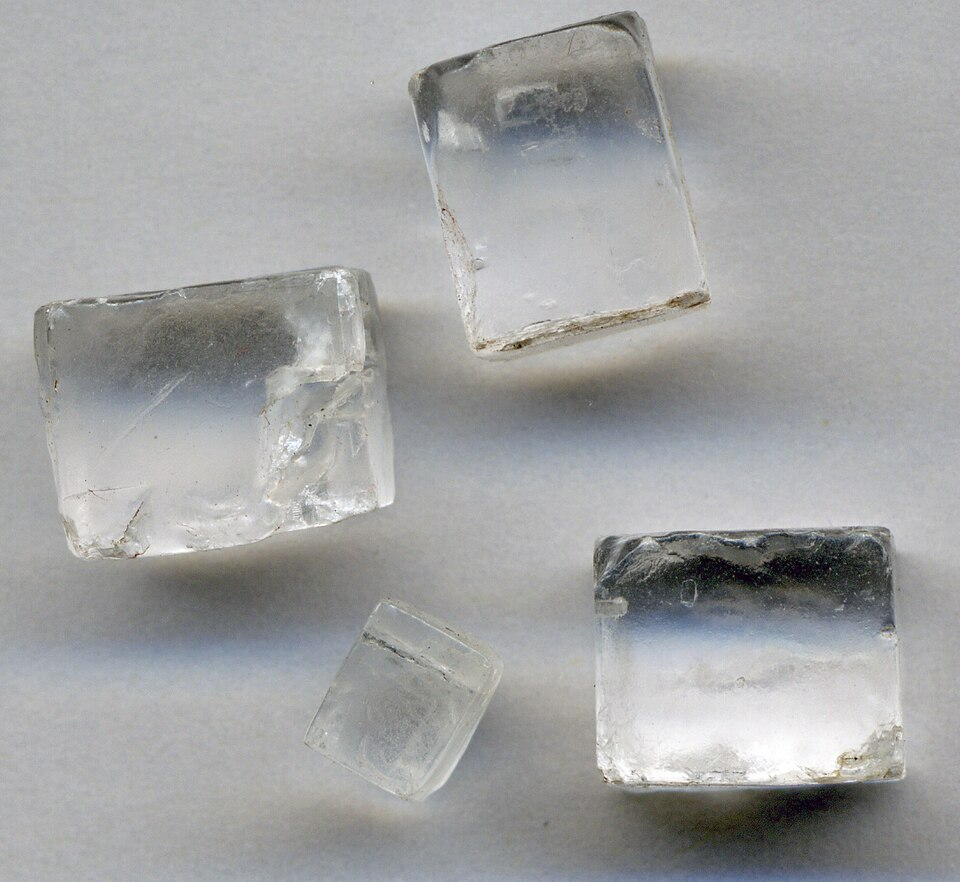
\includegraphics[width=\linewidth]{images/book2/halite.jpg}

{\small \omterm{def:b1:crystals-metals:crystal}{Cristales} de halita (sal gema). Foto: James St. John, CC BY 2.0.}
\end{minipage}\hfill
\begin{minipage}[b]{0.31\linewidth}\centering
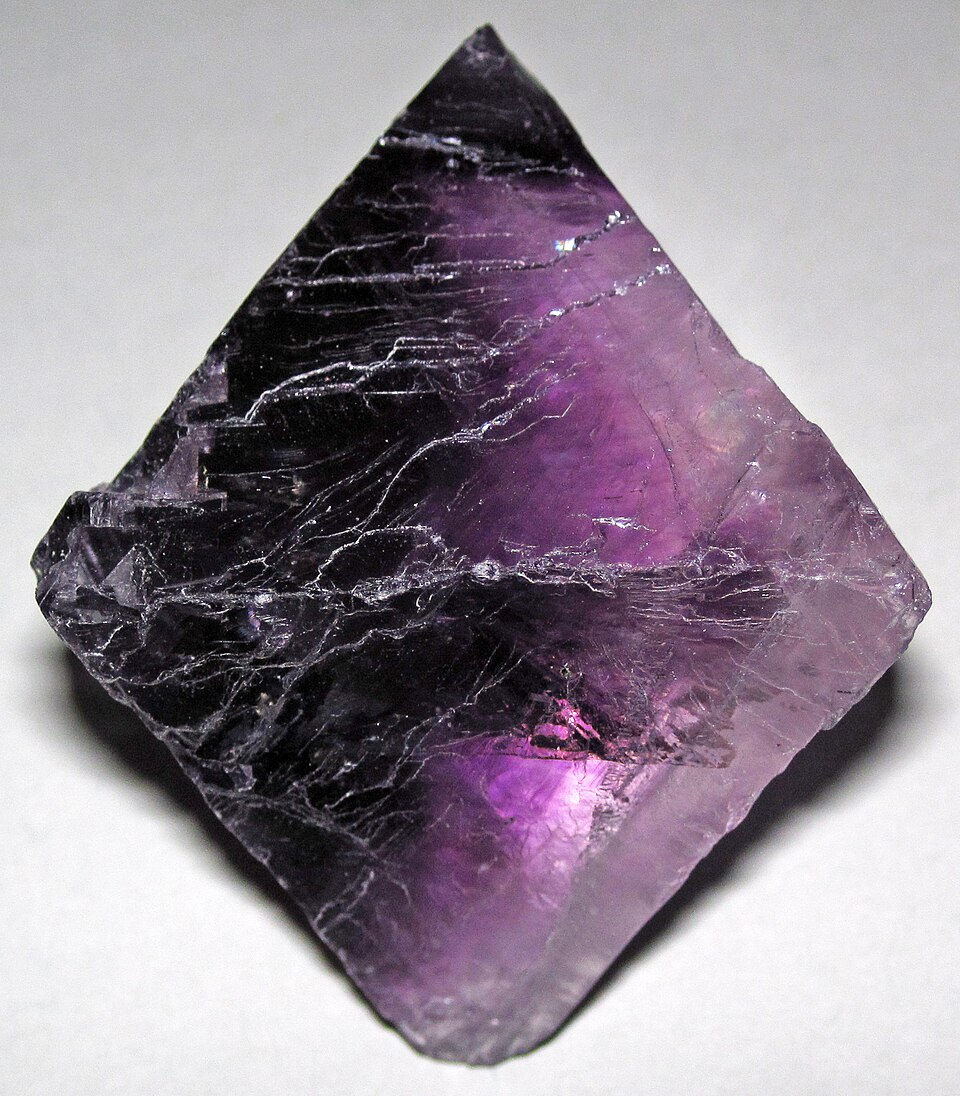
\includegraphics[width=0.85\linewidth]{images/book2/fluorite.jpg}

{\small Fluorita, \ce{CaF2}. Foto: James St. John, CC BY 2.0.}
\end{minipage}\hfill
\begin{minipage}[b]{0.31\linewidth}\centering
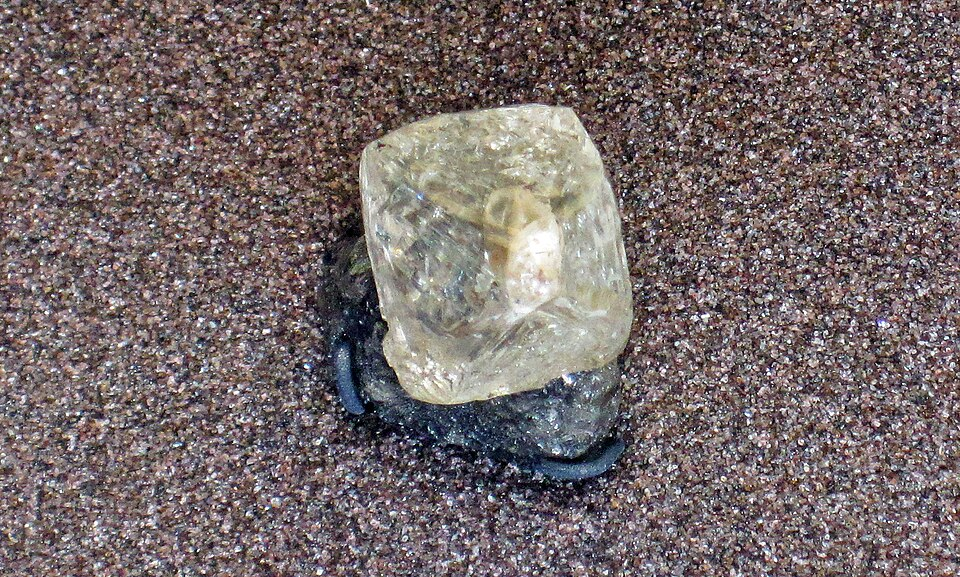
\includegraphics[width=\linewidth]{images/book2/diamond.jpg}

{\small Un octaedro de diamante en bruto. Foto: James St. John, CC BY 2.0.}
\end{minipage}
\end{omfigure}

\begin{proposition}[Tipos blenda y fluorita]\label{prop:b1:crystals-ionic-covalent:zns-caf2}
En el \omterm{def:b1:crystals-ionic-covalent:structure-type}{tipo blenda}, $Z = 4$, cada ion está rodeado por cuatro del otro
tipo en los vértices de un tetraedro, y los iones se tocan a lo largo de
un cuarto de la diagonal principal: $a\sqrt3/4 = r_+ + r_-$. En el \omterm{def:b1:crystals-ionic-covalent:structure-type}{tipo
fluorita} hay $Z = 4$ unidades \ce{CaF2}; cada catión tiene 8 aniones
vecinos (un cubo), cada anión 4 cationes vecinos (un tetraedro), y de
nuevo $a\sqrt3/4 =
r_+ + r_-$.
\end{proposition}

\begin{proof}
Blenda: 4 aniones en la \omterm{def:b1:crystals-metals:lattice}{red} FCC y 4 cationes en la mitad de los 8 \omterm{def:b1:crystals-metals:site}{huecos
tetraédricos}. Un \omterm{def:b1:crystals-metals:site}{hueco tetraédrico} en $(\frac a4,\frac a4,\frac a4)$ está
a $\frac{a\sqrt3}{4}$ de sus cuatro aniones. Fluorita: 4 cationes y 8
aniones en todos los \omterm{def:b1:crystals-metals:site}{huecos tetraédricos}, proporción $1:2$. Los 8 aniones
del interior de la celda forman un cubo de arista $a/2$, y de los cubos
de aniones uno de cada dos aloja un catión en su centro; un anión tiene
sus 4 cationes vecinos a $\frac{a\sqrt3}{4}$.
\end{proof}

\begin{omfigure}
\tdplotsetmaincoords{60}{100}
\begin{tikzpicture}[tdplot_main_coords, font=\small]
  \pic {omcubeo={3}};
  \begin{scope}[on background layer]
    \draw[black!45, line width=1.2pt] (0.75,0.75,2.25) -- (0,0,3) (0.75,0.75,2.25) -- (0,1.5,1.5) (0.75,0.75,2.25) -- (1.5,0,1.5) (0.75,0.75,2.25) -- (1.5,1.5,3) (0.75,2.25,0.75) -- (0,1.5,1.5) (0.75,2.25,0.75) -- (0,3,0) (0.75,2.25,0.75) -- (1.5,1.5,0) (0.75,2.25,0.75) -- (1.5,3,1.5) (2.25,0.75,0.75) -- (1.5,0,1.5) (2.25,0.75,0.75) -- (1.5,1.5,0) (2.25,0.75,0.75) -- (3,0,0) (2.25,0.75,0.75) -- (3,1.5,1.5) (2.25,2.25,2.25) -- (1.5,1.5,3) (2.25,2.25,2.25) -- (1.5,3,1.5) (2.25,2.25,2.25) -- (3,1.5,1.5) (2.25,2.25,2.25) -- (3,3,3);
  \end{scope}
    \node[aX={yellow!75!orange}{6mm}] at (0,0,0) {};
  \node[aX={yellow!75!orange}{6mm}] at (0,3,0) {};
  \node[aX={yellow!75!orange}{6mm}] at (0,1.5,1.5) {};
  \node[aX={gray!60}{3.6mm}] at (0.75,2.25,0.75) {};
  \node[aX={yellow!75!orange}{6mm}] at (0,0,3) {};
  \node[aX={yellow!75!orange}{6mm}] at (1.5,1.5,0) {};
  \node[aX={gray!60}{3.6mm}] at (0.75,0.75,2.25) {};
  \node[aX={yellow!75!orange}{6mm}] at (0,3,3) {};
  \node[aX={yellow!75!orange}{6mm}] at (1.5,0,1.5) {};
  \node[aX={gray!60}{3.6mm}] at (2.25,0.75,0.75) {};
  \node[aX={yellow!75!orange}{6mm}] at (1.5,3,1.5) {};
  \node[aX={yellow!75!orange}{6mm}] at (3,0,0) {};
  \node[aX={yellow!75!orange}{6mm}] at (1.5,1.5,3) {};
  \node[aX={yellow!75!orange}{6mm}] at (3,3,0) {};
  \node[aX={gray!60}{3.6mm}] at (2.25,2.25,2.25) {};
  \node[aX={yellow!75!orange}{6mm}] at (3,1.5,1.5) {};
  \node[aX={yellow!75!orange}{6mm}] at (3,0,3) {};
  \node[aX={yellow!75!orange}{6mm}] at (3,3,3) {};
  \node at (1.5,1.5,-1.75) {\ce{ZnS} (blenda)};
\end{tikzpicture}
\hspace{1cm}
\begin{tikzpicture}[tdplot_main_coords, font=\small]
  \pic {omcubeo={3}};
    \node[aX={green!35!gray}{4.4mm}] at (0,0,0) {};
  \node[aX={green!35!gray}{4.4mm}] at (0,3,0) {};
  \node[aX={green!35!gray}{4.4mm}] at (0,1.5,1.5) {};
  \node[aX={green!45!yellow}{5.0mm}] at (0.75,0.75,0.75) {};
  \node[aX={green!45!yellow}{5.0mm}] at (0.75,2.25,0.75) {};
  \node[aX={green!35!gray}{4.4mm}] at (0,0,3) {};
  \node[aX={green!35!gray}{4.4mm}] at (1.5,1.5,0) {};
  \node[aX={green!45!yellow}{5.0mm}] at (0.75,0.75,2.25) {};
  \node[aX={green!35!gray}{4.4mm}] at (0,3,3) {};
  \node[aX={green!35!gray}{4.4mm}] at (1.5,0,1.5) {};
  \node[aX={green!45!yellow}{5.0mm}] at (0.75,2.25,2.25) {};
  \node[aX={green!45!yellow}{5.0mm}] at (2.25,0.75,0.75) {};
  \node[aX={green!35!gray}{4.4mm}] at (1.5,3,1.5) {};
  \node[aX={green!35!gray}{4.4mm}] at (3,0,0) {};
  \node[aX={green!45!yellow}{5.0mm}] at (2.25,2.25,0.75) {};
  \node[aX={green!35!gray}{4.4mm}] at (1.5,1.5,3) {};
  \node[aX={green!35!gray}{4.4mm}] at (3,3,0) {};
  \node[aX={green!45!yellow}{5.0mm}] at (2.25,0.75,2.25) {};
  \node[aX={green!45!yellow}{5.0mm}] at (2.25,2.25,2.25) {};
  \node[aX={green!35!gray}{4.4mm}] at (3,1.5,1.5) {};
  \node[aX={green!35!gray}{4.4mm}] at (3,0,3) {};
  \node[aX={green!35!gray}{4.4mm}] at (3,3,3) {};
  \node at (1.5,1.5,-1.75) {\ce{CaF2} (fluorita)};
\end{tikzpicture}

{\small A la izquierda, la blenda, con \ce{S^{2-}} (amarillo) en una \omterm{def:b1:crystals-metals:lattice}{red}
FCC y \ce{Zn^{2+}} (gris) en \omterm{def:b1:crystals-metals:site}{huecos tetraédricos} alternos, cada uno unido
a sus cuatro vecinos. A la derecha, la fluorita, con \ce{Ca^{2+}} (verde
grisáceo) en una \omterm{def:b1:crystals-metals:lattice}{red} FCC y \ce{F-} (verde claro) en los ocho \omterm{def:b1:crystals-metals:site}{huecos
tetraédricos}.}
\end{omfigure}

\begin{example}[Blenda y fluorita]\label{ex:b1:crystals-ionic-covalent:zns}
La blenda tiene $a = \qty{540.9}{pm}$: $r_+ + r_- = a\sqrt3/4 =
\qty{234.2}{pm}$ (Shannon: $60 + 184 = \qty{244}{pm}$, pues el radio del
sulfuro solo está tabulado para seis vecinos), y $x = 60/184 = 0.33$, en
el intervalo tetraédrico. La fluorita tiene $a = \qty{546.3}{pm}$:
$r_+ + r_- =
\qty{236.6}{pm}$ (Shannon: $112 + 131 = \qty{243}{pm}$), y $x = 0.85$:
el catión se sitúa en un cubo de 8 aniones, como exige la regla.
% ledger: lat:ZnS, rion:Zn2+IV, rion:S2-VI, lat:CaF2, rion:Ca2+VIII,
% rion:F-IV
\end{example}

\begin{method}[Predecir una estructura]\label{met:b1:crystals-ionic-covalent:predict}
Para predecir la estructura de un compuesto iónico \ce{MX} o \ce{MX2}:
\begin{enumerate}
  \item se calcula $x = r_+/r_-$ con radios tabulados (para la
        coordinación esperada);
  \item se lee la coordinación del catión en la regla de la \omterm{def:b1:crystals-ionic-covalent:radius-ratio}{relación de
        radios};
  \item se elige el tipo que tiene esa coordinación y la fórmula
        adecuada: \ce{MX} con 8, \ce{CsCl}; con 6, \ce{NaCl}; con 4,
        blenda; \ce{MX2} con 8, fluorita;
  \item se contrasta con el parámetro de \omterm{def:b1:crystals-metals:lattice}{red} medido, recordando que los
        iones polarizables (\ce{S^{2-}}, \ce{I-}) y los cationes pequeños
        y cargados dan enlaces parcialmente covalentes, para los que la
        regla falla.
\end{enumerate}
\end{method}

\section{Cristales covalentes}

\begin{definition}[Cristal covalente]\label{def:b1:crystals-ionic-covalent:covalent-crystal}
Un \emph{cristal covalente}\index{cristal covalente} (o sólido reticular)
es un \omterm{def:b1:crystals-metals:crystal}{cristal} en el que todos los átomos están unidos por \omterm{def:b1:lewis-resonance-vsepr:lewis}{enlaces
covalentes} en una única molécula gigante: el diamante, el silicio, el
cuarzo \ce{SiO2}. En un \omterm{def:b1:crystals-metals:crystal}{cristal} covalente laminar como el grafito, la red
covalente solo se extiende en planos, que se mantienen unidos entre sí
por \omterm{def:b1:intermolecular-forces-solvents:vdw}{interacciones de van der Waals}.
\end{definition}

\begin{proposition}[La estructura del diamante]\label{prop:b1:crystals-ionic-covalent:diamond}
En el diamante, los átomos de carbono ocupan la \omterm{def:b1:crystals-metals:lattice}{red} FCC y la mitad de sus
\omterm{def:b1:crystals-metals:site}{huecos tetraédricos}, como los dos tipos de iones de la blenda: $Z = 8$, y
cada carbono está unido a otros cuatro situados en los vértices de un
tetraedro, a la distancia $a\sqrt3/4$. Para esferas en contacto, la
\omterm{def:b1:crystals-metals:compactness}{compacidad} es
\[
  C = \frac{\pi\sqrt3}{16} \approx 0.34 .
\]
\end{proposition}

\begin{proof}
$Z = 4 + 4 = 8$. Los átomos vecinos se tocan: $2R = a\sqrt3/4$, de modo
que $a =
8R/\sqrt3$ y $C = 8 \cdot \frac43\pi R^3/a^3 = \frac{32}{3}\pi R^3 \cdot
\frac{3\sqrt3}{512 R^3} = \frac{\pi\sqrt3}{16}$.
\end{proof}

\begin{omfigure}
\tdplotsetmaincoords{60}{100}
\begin{tikzpicture}[tdplot_main_coords, font=\small]
  \pic {omcubeo={3}};
  \begin{scope}[on background layer]
    \draw[black!55, line width=1.4pt] (0.75,0.75,2.25) -- (0,0,3) (0.75,0.75,2.25) -- (0,1.5,1.5) (0.75,0.75,2.25) -- (1.5,0,1.5) (0.75,0.75,2.25) -- (1.5,1.5,3) (0.75,2.25,0.75) -- (0,1.5,1.5) (0.75,2.25,0.75) -- (0,3,0) (0.75,2.25,0.75) -- (1.5,1.5,0) (0.75,2.25,0.75) -- (1.5,3,1.5) (2.25,0.75,0.75) -- (1.5,0,1.5) (2.25,0.75,0.75) -- (1.5,1.5,0) (2.25,0.75,0.75) -- (3,0,0) (2.25,0.75,0.75) -- (3,1.5,1.5) (2.25,2.25,2.25) -- (1.5,1.5,3) (2.25,2.25,2.25) -- (1.5,3,1.5) (2.25,2.25,2.25) -- (3,1.5,1.5) (2.25,2.25,2.25) -- (3,3,3);
  \end{scope}
  \node[aX={black!65}{3.6mm}] at (0,0,0) {};
  \node[aX={black!65}{3.6mm}] at (0,3,0) {};
  \node[aX={black!65}{3.6mm}] at (0,1.5,1.5) {};
  \node[aX={black!65}{3.6mm}] at (0.75,2.25,0.75) {};
  \node[aX={black!65}{3.6mm}] at (0,0,3) {};
  \node[aX={black!65}{3.6mm}] at (1.5,1.5,0) {};
  \node[aX={black!65}{3.6mm}] at (0.75,0.75,2.25) {};
  \node[aX={black!65}{3.6mm}] at (0,3,3) {};
  \node[aX={black!65}{3.6mm}] at (1.5,0,1.5) {};
  \node[aX={black!65}{3.6mm}] at (2.25,0.75,0.75) {};
  \node[aX={black!65}{3.6mm}] at (1.5,3,1.5) {};
  \node[aX={black!65}{3.6mm}] at (3,0,0) {};
  \node[aX={black!65}{3.6mm}] at (1.5,1.5,3) {};
  \node[aX={black!65}{3.6mm}] at (3,3,0) {};
  \node[aX={black!65}{3.6mm}] at (2.25,2.25,2.25) {};
  \node[aX={black!65}{3.6mm}] at (3,1.5,1.5) {};
  \node[aX={black!65}{3.6mm}] at (3,0,3) {};
  \node[aX={black!65}{3.6mm}] at (3,3,3) {};
  \node at (1.5,1.5,-1.75) {diamante};
\end{tikzpicture}
\hspace{0.8cm}
\begin{tikzpicture}[font=\small, y={(0cm,0.45cm)}, z={(0cm,1cm)}, x={(1cm,0cm)}]
  % two honeycomb layers seen in perspective, ABAB stacking
  \foreach \zz/\dy/\col in {0/0/black!40, 1.7/0.82/black!80} {
    \foreach \i in {0,1,2} \foreach \j in {0,1} {
      \pgfmathsetmacro\cx{1.42*\i+0.71*\j}
      \pgfmathsetmacro\cy{1.23*\j+\dy}
      \foreach \k in {0,60,...,300} {
        \pgfmathsetmacro\ka{\k+60}
        \draw[\col, line width=1pt] ({\cx+0.82*cos(\k+30)},{\cy+0.82*sin(\k+30)},\zz)
          -- ({\cx+0.82*cos(\ka+30)},{\cy+0.82*sin(\ka+30)},\zz);
      }
    }
  }
  \draw[<->, omThm] (5.6,0.9,0) -- (5.6,0.9,1.7) node[midway, right] {\qty{335}{pm}};
  \node at (2.4,-1.6,0) {grafito};
\end{tikzpicture}

{\small A la izquierda, la celda del diamante, con cada carbono unido a
otros cuatro en un tetraedro. A la derecha, el grafito, capas de
hexágonos (C--C \qty{141.8}{pm} dentro de una capa) apiladas a
\qty{334.8}{pm} unas de otras y unidas por fuerzas de London; las capas
alternan ABAB.}
% ledger: lat:C-graphite.a, lat:C-graphite.c (C-C = a/sqrt3; interlayer = c/2)
\end{omfigure}

\begin{example}[Diamante, silicio, grafito]\label{ex:b1:crystals-ionic-covalent:carbon}
El diamante tiene $a = \qty{356.7}{pm}$: \ce{C-C} $= a\sqrt3/4 =
\qty{154.5}{pm}$, el enlace sencillo del etano, y $\rho =
\qty{3.52}{g/cm^3}$. El silicio, de la misma estructura con $a =
\qty{543.1}{pm}$, tiene \ce{Si-Si} $= \qty{235.2}{pm}$ y $\rho =
\qty{2.33}{g/cm^3}$ (medida: 2.33). En el grafito, cada carbono está unido
a otros tres en un plano a \qty{141.8}{pm}, un orden de enlace entre uno
y dos (resonancia en toda la capa), mientras que las capas están a
\qty{334.8}{pm} unas de otras. El diamante, rígido en las tres
dimensiones, es el material natural más duro y un aislante; el grafito se
exfolia entre sus capas, que se deslizan con facilidad, y conduce la
electricidad dentro de ellas gracias a sus electrones $\pi$
deslocalizados.
% ledger: lat:C-diamond, lat:Si, rho:Si, lat:C-graphite.a, lat:C-graphite.c,
% geo:C2H6.rCC
\end{example}

\begin{omfigure}
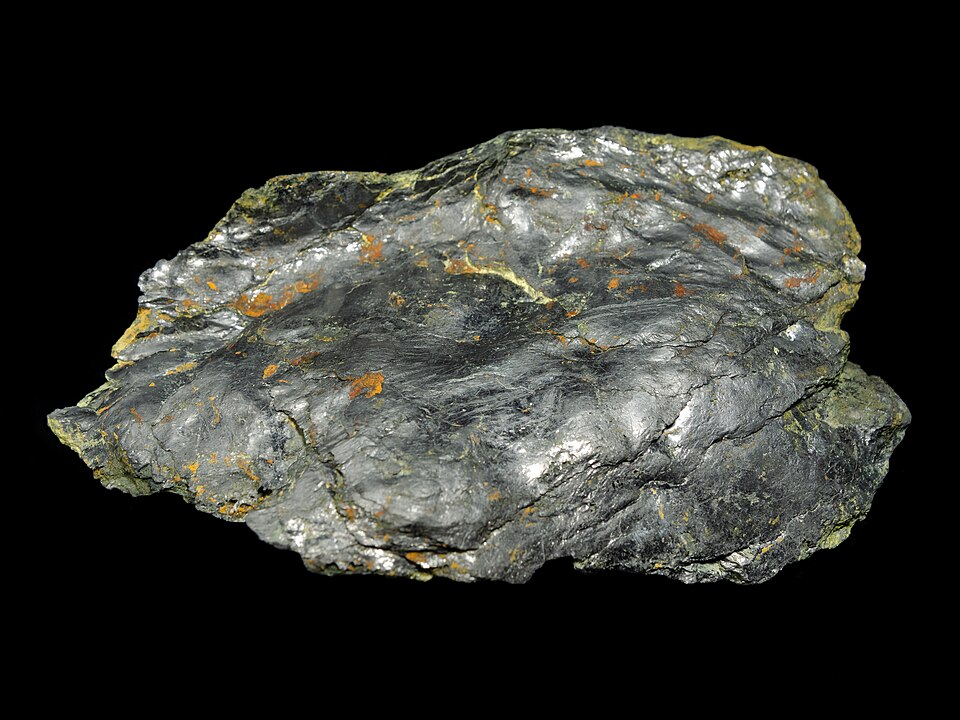
\includegraphics[width=0.36\linewidth]{images/book2/graphite.jpg}

{\small Un ejemplar de grafito natural, con su brillo metálico. Foto:
Zbynek Burival, CC BY-SA 4.0.}
\end{omfigure}

\section{Cristales moleculares}

\begin{definition}[Cristal molecular]\label{def:b1:crystals-ionic-covalent:molecular-crystal}
Un \emph{cristal molecular}\index{cristal molecular} es un \omterm{def:b1:crystals-metals:crystal}{cristal} de
moléculas unidas por fuerzas intermoleculares --- \omterm{def:b1:intermolecular-forces-solvents:vdw}{interacciones de van
der Waals} y, si es posible, \omterm{def:b1:intermolecular-forces-solvents:hbond}{enlaces de hidrógeno} ---, en el que cada
molécula conserva sus propios \omterm{def:b1:lewis-resonance-vsepr:lewis}{enlaces covalentes}: el diyodo, el hielo
seco \ce{CO2(s)}, el hielo, el azúcar.
\end{definition}

\begin{proposition}[Propiedades de los cristales moleculares]\label{prop:b1:crystals-ionic-covalent:molecular}
Los \omterm{def:b1:crystals-ionic-covalent:molecular-crystal}{cristales moleculares} son blandos y funden o subliman a temperaturas
bajas, ya que solo se rompen fuerzas intermoleculares débiles; no
conducen.
\end{proposition}
\admitted

\begin{example}[El hielo]\label{ex:b1:crystals-ionic-covalent:ice}
En el hielo ordinario, cada molécula de agua está unida por \omterm{def:b1:intermolecular-forces-solvents:hbond}{enlaces de
hidrógeno} a otras cuatro situadas en los vértices de un tetraedro: dos
mediante sus propios hidrógenos y dos mediante sus \omterm{def:b1:lewis-resonance-vsepr:lewis}{pares no enlazantes}.
Esta red abierta y hexagonal, impuesta por las direcciones de los \omterm{def:b1:intermolecular-forces-solvents:hbond}{enlaces
de hidrógeno}, deja mucho espacio vacío: el hielo es menos denso que el
agua líquida, en la que la red está parcialmente rota y las moléculas se
acercan más. La simetría hexagonal de la red se manifiesta en la forma
de seis puntas de los \omterm{def:b1:crystals-metals:crystal}{cristales} de nieve.
\end{example}

\begin{omfigure}
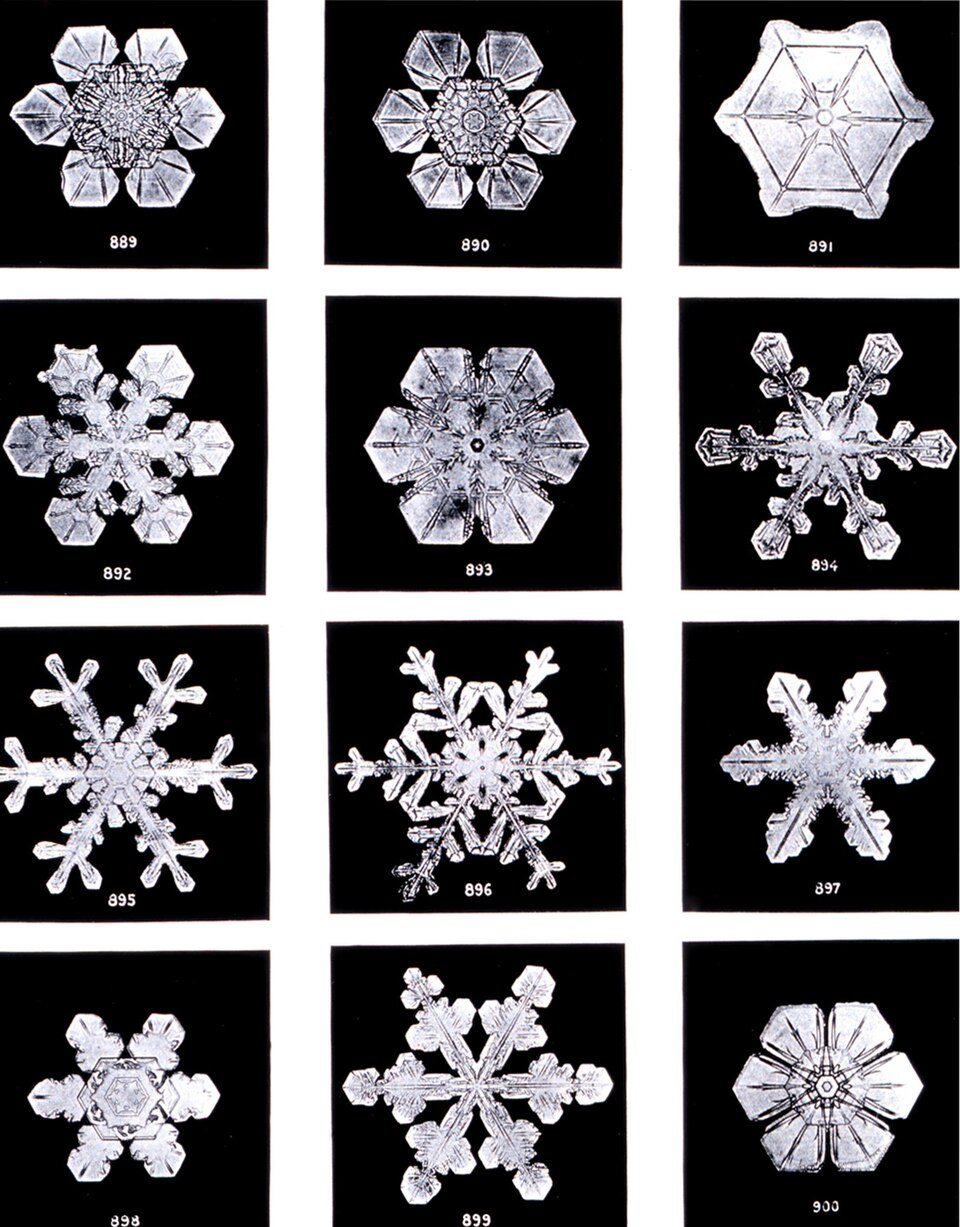
\includegraphics[width=0.38\linewidth]{images/book2/bentley-snowflakes.jpg}

{\small \omterm{def:b1:crystals-metals:crystal}{Cristales} de nieve fotografiados por Wilson Bentley hacia 1902:
todos tienen simetría de orden seis, la huella de la red hexagonal de
\omterm{def:b1:intermolecular-forces-solvents:hbond}{enlaces de hidrógeno} del hielo. Dominio público.}
\end{omfigure}

\section{Comparación de los cuatro tipos de sólidos}

\begin{center}
\small
\begin{tabular}{lllll}
\hline
sólido & partículas & cohesión & propiedades & ejemplos \\
\hline
metálico & cationes, electrones & \omterm{def:b1:crystals-metals:metallic-bond}{enlace metálico} & conductor, dúctil & \ce{Cu}, \ce{Fe}, \ce{Na} \\
iónico & cationes, aniones & electrostática & duro, frágil, aislante & \ce{NaCl}, \ce{CaF2} \\
covalente & átomos & \omterm{def:b1:lewis-resonance-vsepr:lewis}{enlaces covalentes} & muy duro, funde alto & diamante, \ce{SiO2} \\
molecular & moléculas & van der Waals, enlaces H & blando, funde bajo & \ce{I2}, hielo \\
\hline
\end{tabular}
\end{center}

\begin{remark}[Un continuo]\label{rem:b1:crystals-ionic-covalent:continuum}
Las clases son idealizaciones. El sulfuro de cinc tiene enlaces en parte
iónicos y en parte covalentes, por lo que su distancia sulfuro--cinc es
más corta que la suma de los \omterm{def:b1:periodicity:radius}{radios iónicos}; el grafito es covalente en
sus capas y molecular entre ellas. La diferencia de \omterm{def:b1:periodicity:electronegativity}{electronegatividad}
(\cref{prop:b1:periodicity:en-trend}) sirve de guía: cuanto mayor es, más
iónico es el sólido.
\end{remark}

\section{Ejercicios}

\begin{exercise}[$\star$]\label{exo:b1:crystals-ionic-covalent:1}
En la celda de la sal gema, cuéntense los cationes y los aniones, dese la
coordinación de cada uno y compruébese que se respeta la fórmula
\ce{NaCl}.
\end{exercise}

\begin{exercise}[$\star$]\label{exo:b1:crystals-ionic-covalent:2}
El cloruro de cesio tiene $a = \qty{412.3}{pm}$. Calcúlense la distancia
\ce{Cs-Cl} más corta y el número de unidades fórmula por celda.
\end{exercise}

\begin{exercise}[$\star$]\label{exo:b1:crystals-ionic-covalent:3}
Con los radios $r(\ce{Na+}) = \qty{102}{pm}$ y $r(\ce{Cl-}) =
\qty{181}{pm}$, calcúlese la \omterm{def:b1:crystals-ionic-covalent:radius-ratio}{relación de radios} de \ce{NaCl} y predígase
la coordinación del catión.
\end{exercise}

\begin{exercise}[$\star$]\label{exo:b1:crystals-ionic-covalent:4}
Clasifíquense como metálicos, iónicos, covalentes o moleculares: el
cobre, el cloruro de sodio, el diamante, el diyodo, el cuarzo \ce{SiO2},
el hielo y el fluoruro de calcio.
\end{exercise}

\begin{exercise}[$\star\star$]\label{exo:b1:crystals-ionic-covalent:5}
Demuéstrese que la estructura de la sal gema exige $r_+/r_- \ge \sqrt2 - 1$.
\end{exercise}

\begin{exercise}[$\star\star$]\label{exo:b1:crystals-ionic-covalent:6}
Calcúlese la densidad del cloruro de sodio a partir de
$a = \qty{564.1}{pm}$ ($M(\ce{NaCl}) = \qty{58.44}{g/mol}$) y compárese
con \qty{2.17}{g/cm^3}.
\end{exercise}

\begin{exercise}[$\star\star$]\label{exo:b1:crystals-ionic-covalent:7}
Calcúlese la densidad del cloruro de cesio ($M = \qty{168.36}{g/mol}$,
$a = \qty{412.3}{pm}$) y compárese con el valor medido,
\qty{3.99}{g/cm^3}.
% ledger: rho:CsCl
\end{exercise}

\begin{exercise}[$\star\star$]\label{exo:b1:crystals-ionic-covalent:8}
Para la blenda ($a = \qty{540.9}{pm}$, $M = \qty{97.44}{g/mol}$),
calcúlense la distancia \ce{Zn-S} y la densidad, y compárese con el valor
medido, \qty{4.04}{g/cm^3}.
% ledger: rho:ZnS
\end{exercise}

\begin{exercise}[$\star\star$]\label{exo:b1:crystals-ionic-covalent:9}
El grafito tiene una celda hexagonal con $a = \qty{245.6}{pm}$ y
$c = \qty{669.6}{pm}$, que contiene 4 átomos. Calcúlense la distancia
\ce{C-C} dentro de una capa ($a/\sqrt3$), la distancia entre capas
($c/2$) y la densidad. ¿Por qué el grafito es menos denso que el
diamante?
\end{exercise}

\begin{exercise}[$\star\star\star$]\label{exo:b1:crystals-ionic-covalent:10}
Demuéstrese que la \omterm{def:b1:crystals-metals:compactness}{compacidad} del diamante es $\pi\sqrt3/16$, y
explíquese por qué el material más duro es uno de los menos compactos.
\end{exercise}

\begin{exercise}[$\star\star\star$]\label{exo:b1:crystals-ionic-covalent:11}
El silicio tiene la estructura del diamante con $a = \qty{543.1}{pm}$.
Calcúlense la longitud del enlace \ce{Si-Si}, el \omterm{def:b1:periodicity:radius}{radio covalente} del
silicio y la densidad ($M = \qty{28.09}{g/mol}$); compárese con
\qty{2.33}{g/cm^3}.
\end{exercise}

\begin{exercise}[$\star\star\star$]\label{exo:b1:crystals-ionic-covalent:12}
El cloruro de rubidio tiene $r(\ce{Rb+}) = \qty{152}{pm}$ (seis vecinos)
y $r(\ce{Cl-}) = \qty{181}{pm}$. ¿Qué estructura predice la regla de la
\omterm{def:b1:crystals-ionic-covalent:radius-ratio}{relación de radios}? En condiciones ordinarias es del \omterm{def:b1:crystals-ionic-covalent:structure-type}{tipo sal gema} con
$a = \qty{658.1}{pm}$: compruébese la distancia \ce{Rb-Cl} y propóngase
por qué falla aquí la regla.
% ledger: rion:Rb+VI, rion:Cl-VI, lat:RbCl
\end{exercise}

\section{Problema: la fluorita, el mineral y la lente}

\begin{problem}[{Problema de fin de semana --- la celda de la fluorita, su
\omterm{def:b1:crystals-ionic-covalent:radius-ratio}{relación de radios}, dos parientes (\ce{Li2O} y el diamante) y la densidad
de la fluorita calculada a partir de su celda}]
\label{pb:b1:crystals-ionic-covalent:1}
La fluorita, \ce{CaF2}, es un mineral; crecida en grandes \omterm{def:b1:crystals-metals:crystal}{cristales}
transparentes, sirve para fabricar lentes que transmiten la luz
ultravioleta. Su celda es cúbica, $a =
\qty{546.3}{pm}$; \ce{Ca^{2+}} en una \omterm{def:b1:crystals-metals:lattice}{red} FCC y \ce{F-} en los \omterm{def:b1:crystals-metals:site}{huecos
tetraédricos}. Radios: $r(\ce{Ca^{2+}}) = \qty{112}{pm}$ (ocho vecinos),
$r(\ce{F-}) = \qty{131}{pm}$ (cuatro vecinos). Masas molares (g/mol):
\ce{Ca} 40.08, \ce{F} 19.00, \ce{Li} 6.94, \ce{O} 16.00, \ce{C}
12.01, \ce{Si} 28.09; $N_A = \qty{6.022e23}{mol^{-1}}$.
% ledger: lat:CaF2, rion:Ca2+VIII, rion:F-IV, aw:Ca, aw:F, aw:Li, aw:O,
% aw:C, aw:Si, const:NA

\medskip
\noindent\textbf{Parte I --- La celda.}
\begin{enumerate}
  \item Dense las posiciones de los iones \ce{Ca^{2+}} en la celda y
        cuéntense.
  \item ¿Cuántos \omterm{def:b1:crystals-metals:site}{huecos tetraédricos} contiene la celda? Dedúzcase el
        número de iones \ce{F-} y compruébese la fórmula.
  \item ¿Cuál es la coordinación de \ce{F-}? ¿Y la de \ce{Ca^{2+}}?
  \item Calcúlese la distancia \ce{Ca-F} más corta.
  \item Compárese con la suma de los \omterm{def:b1:periodicity:radius}{radios iónicos}.
  \item Calcúlese la distancia \ce{F-F} más corta y dígase si los aniones
        se tocan.
\end{enumerate}

\medskip
\noindent\textbf{Parte II --- La \omterm{def:b1:crystals-ionic-covalent:radius-ratio}{relación de radios}.}
\begin{enumerate}[resume]
  \item Calcúlese $x = r_+/r_-$.
  \item ¿Qué coordinación del catión permite la regla de la \omterm{def:b1:crystals-ionic-covalent:radius-ratio}{relación de
        radios}?
  \item ¿Por qué \ce{CaF2} no puede adoptar la estructura del cloruro de
        cesio, aunque su catión tenga coordinación 8?
  \item Descríbase la fluorita como una disposición cúbica simple de
        \ce{F-} con \ce{Ca^{2+}} en los centros de la mitad de los cubos
        pequeños.
  \item Calcúlese la \omterm{def:b1:crystals-metals:compactness}{compacidad} de la fluorita.
\end{enumerate}

\medskip
\noindent\textbf{Parte III --- Dos parientes.}
El óxido de litio, \ce{Li2O}, es de \omterm{def:b1:crystals-ionic-covalent:structure-type}{tipo antifluorita} con
$a = \qty{461.9}{pm}$; $r(\ce{Li+}) = \qty{59}{pm}$ (cuatro vecinos),
$r(\ce{O^{2-}}) =
\qty{142}{pm}$ (ocho vecinos). Diamante: $a = \qty{356.7}{pm}$.
% ledger: lat:Li2O, rion:Li+IV, rion:O2-VIII, rho:Li2O, lat:C-diamond
\begin{enumerate}[resume]
  \item ¿Dónde están los iones \ce{O^{2-}} y \ce{Li+} en la celda de la
        antifluorita?
  \item Calcúlese la distancia \ce{Li-O} y compárese con la suma de los
        radios.
  \item Calcúlese la densidad de \ce{Li2O} y compárese con el valor
        medido, \qty{2.01}{g/cm^3}.
  \item ¿Qué estructura iónica tiene la misma disposición de posiciones
        que el diamante?
  \item Calcúlense la longitud del enlace \ce{C-C} y la densidad del
        diamante.
  \item ¿Por qué el diamante es mucho menos compacto que la fluorita,
        aunque sus átomos ocupen el mismo tipo de posiciones?
\end{enumerate}

\medskip
\noindent\textbf{Parte IV --- La densidad de la fluorita.}
\begin{enumerate}[resume]
  \item Calcúlese la masa molar de \ce{CaF2}.
  \item Calcúlese la masa de una celda.
  \item Calcúlese el volumen de una celda, en \unit{cm^3}.
  \item ¿Qué efecto tendría sobre la densidad una vacante en una posición
        de \ce{F-} de cada cien celdas?
  \item Calcúlese la densidad de la fluorita a partir de su celda y
        compárese con el valor medido, \qty{3.18}{g/cm^3}.
\end{enumerate}
% ledger: rho:CaF2
\end{problem}
